%----------------------------------------------------------------------------   
\chapter{Felhő alapú VoIP médiasík}
%---------------------------------------------------------------------------- 

\section{Kubernetes telepítése}

A Kubernetes architektúra tervezése során a fő szempont az volt, hogy teljes mértékben 
úgy nézzen ki kívülről, mintha egy szimpla rtpengine lenne. De mögötte egy 
mikroszolgáltatásokból álló alkalmazás legyen, mely képes az benne rejlő rtpengine-t 
megfelelően konfigurálni.

Ezt a Kubernetes klasztert a BME által szolgáltatott szervereken építettem ki, mi szám 
szerint 4 szervert tartalmaz melyek az \ref{fig:servers} elrendezésben vannak összekötve.

\begin{figure}[!ht]
	\centering
	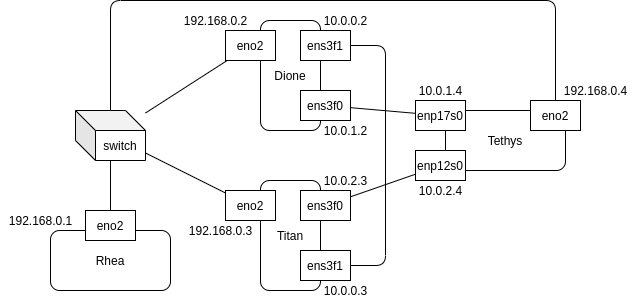
\includegraphics[width=1\textwidth, keepaspectratio]{figures/servers.png}
	\caption{Szerverek összeköttetése}
	\label{fig:servers}
\end{figure}

Az ábrán szereplő szervereket kettő részre lehet szétbontani, ahol az egyik
konkrétan a Kubernetes klaszter a másik pedig a forgalom generálására használatos.
Az előbbibe tartozik a \texttt{Rhea}, mint mester csomópont és dolgozó csomópontok közé 
a \texttt{Dione} és a \texttt{Titan}. Majd értelemszerűen az utóbbiba tartozik a 
\texttt{Tethys}. 

A szerverek között a kapcsolatot a vonalakkal jeleztem, melyek, mint látszik
sok esetben direkt összeköttetésben vannak egymással. Ez azért van, mert ezek
az interfészek 40 gigabitesek és az egyetemen nem állt rendelkezésre ilyen 
sebességű switch. Ezáltal a Kubernetes klaszter telepítése során különös figyelmet
kellett szentelni annak, hogy ezek az interfészek helyesen legyenek felkonfigurálva.

De, mint látszik a hálózatban szerepel egy switch, amibe az \texttt{eno2} interfészek 
vannak becsatlakoztatva. Ezek az interfészek 1 gigabites sebességgel rendelkeznek, amik
a sok nagy sebességű forgalmat nem képes kiszolgálni, viszont még így is hasznosak
a hálózat szempontjából. Mivel a telepített Kubernetes klaszter vezérlő- és adatsíkja
ezen a két összeköttetésen osztozik. Szóval a lassabb interfészeken kommunikál az
API szerver és a Kubelet, míg a Kube-Proxy a nagy sebességű hálózati kártyákat 
használja. Ezáltal lehetett egy olyan magas határt szabni a lehetséges forgalom
sebességének, amibe nehéz beleütközni. 

Ahhoz, hogy az előzőleg leírt hálózat elkülönítés működjön a Kuberspray programot 
használtam, mert ennél könnyedén lehetett a telepítés során kettő különböző interfészt
beállítani. A Kuberspray \cite{kubespray} programmal Kubernetes klasztereket lehet 
telepíteni szimplán szerverekre. A különlegessége az, hogy Ansible-t használ erre a 
célra. Szóval elég a mester szerver számára lehetővé tenni, hogy működjön az \texttt{ssh} 
a többi szerverrel és egyetlen konfigurációs fájl indításával képes minden szükséges 
szoftvert feltelepíteni és azokat beállítani. Az Ansible \cite{ansible} nagyjából 
bármilyen folyamatot tud automatizálni a szerverek között. 

\section{Kubernetes architektúra}

A címben említett architektúra írja le, hogy a Kubernetes klasztereken belül milyen 
Kubernetes erőforrások találhatóak meg és azok, hogyan vannak egymással összekötve. A 
\ref{fig:clusterSetup} ábrát kifejtve lehet ezt legjobban elmagyarázni. Fontos 
megjegyezni, hogy erre a rengeteg átalakításra azért van szükség, mert a Kamailio 
legfrissebb stabil verziója nem tud WebSocket-n keresztül vezérlőcsomagokat küldeni és az 
rtpengine-nek az a verziója, amivel a Redis-t ilyen módon lehet használni nem támogatja 
szintúgy a WebSocket-t. Viszont szükség van a WebSocket-re, ami a későbbiekben kifejtésre 
kerül.

\begin{figure}[!ht]
	\centering
	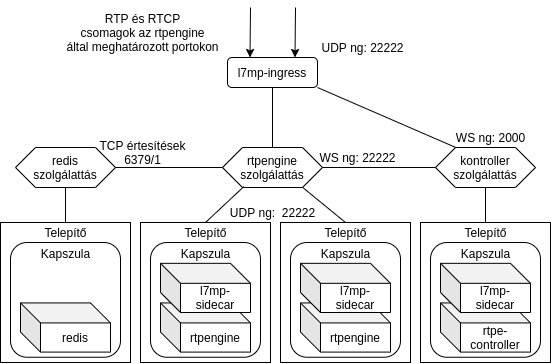
\includegraphics[width=1\textwidth, keepaspectratio]{figures/cluster.png}
	\caption{Kubernetes klaszter felépítése}
	\label{fig:clusterSetup}
\end{figure}

\subsection{Ingress}

Mint látszik a hálózatba való belépés az \texttt{l7mp-ingress} kapun történik, ahol 
kezdetben statikusan konfigurálva van egy figyelő, ami a dolgozó csomópont 22222 UDP 
portján vár minden az rtpengine-nek szánt vezérlőüzenetet. De látszik, hogy a kontroller 
szolgáltatás a 2000-s WebSocket porton várja az üzeneteket. Ezért az 
\texttt{l7mp-ingress} ezen figyelőjének tudnia kell UDP csomagokat WebSocket-re 
átalakítani. Ez az L7mp-nek köszönhetően nagyon egyszerűen megvalósítható volt ugyanis, 
elég csak egy UDP figyelőt létrehozni majd azt egy WebSocket L7mp klaszterekhez 
irányítani, aminek a végpontja a kontroller szolgáltatás. 

\subsection{Kontroller}

A munkám jelentős része ennek a kontrollernek az elkészítése volt, amit ebben a
fejezetben csak annyira ismertetek, hogy kiderüljön a szerepe a \ref{fig:clusterSetup}
ábrán szereplő architektúrában. Részletesen a \ref{sec:controller} fejezetben kerül 
kifejtésre. 

A kontroller a beérkező vezérlőüzeneteket automatikusan továbbítja az rtpengine 
szolgáltatásnak WebSocket-en keresztül. Mielőtt fojtatnám azzal, hogy a kontroller milyen 
feladatokat lát el fontos kifejteni a WebSocket protokoll szükségességét ebben az esetben.
Mivel minden WebSocket csomag rendelkezik egy HTTP-hez hasonló fejléccel így
lehet egyéni információkat küldeni fejlécekben. Ez az információ ebben az esetben a 
híváshoz tartozó  két azonosítót jelent. Az egyik a hívásazonosító míg a másik a hívásban 
résztvevő fél forrásazonosítója. Mivel ez a kettő információ fog szerepelni minden 
csomagban így elérhető az, hogy a vezérlő üzenetek mindig ugyanahhoz a kapszulához 
jussanak el.  Megakadályozva azt az esetet, amikor az \texttt{answer} és \texttt{offer} 
két különböző rtpengine kapszulához jut el, ami miatt nem tud kiépülni rendesen a hívás. 
Ennek elkerülésére a kontroller pótkocsijában kettő figyelőnek kell szerepelnie az egyik 
az \texttt{l7mp-ingress}-től várja a vezérlőüzeneteket és a másikon a helyi hálózatról 
várja azokat az üzeneteket, amiket el kell küldenie az rtpengine felé. 

De visszatérve arra, hogy a kontrollerre miért is van szükség. A kontrollernek két fő 
feladata van. Az első, hogy a hívásokhoz szükséges CRD-ket létrehozza és törölje, így az 
L7mp operátor tudni fogja, hogy milyen beállításokat kell alkalmaznia az L7mp proxy 
pótkocsikban. Aztán van a másik feladata, amivel a kimenő üzeneteket kell átírni annak 
megfelelően, hogy a dolgozó csomópont címe legyen benne és ne \texttt{127.0.0.1}, mert az 
rtpengine mindig ezt a címet fogja beletenni a módosított SDP üzenetekbe. 

\subsection{rtpengine}\label{sec:rtpengine}

Az rtpengine ebben az esetben teljesen ugyanazt a funkciót látja el, mint egy normális 
hívás esetében azzal a különbséggel, hogy képes redundánsan működni. Szóval, ha az 
egyiken létrejön egy hívás, akkor az létezni fog a másikon is és képes rögtön kezelni a 
beérkező forgalmat. Ezt oly módon teszi, hogy minden híváshoz létrehoz egy rekordot a 
Redis adatbázisban, ami keyspace-ket (kulcshelyeket) használ. Azért van szükség arra, 
hogy kulcshely tábla legyen használva az adatbázisban, mert erre fel lehet iratkozni. 
Szóval a két rtpengine kapszula feliratkozik ugyanarra a kulcshelyre, ahova mind a két 
kapszula fogja írni a beérkező hívásaikat. Tehát, ha az egyik kapott egy hívást az 
létrehoz egy rekordot az adott kulcshelyen, amiről a Redis értesíti a másik kapszulát és 
elküldi annak ezeket az információkat, ami majd létrehozza az adott hívást és kinyitja az 
hozzá szükséges portokat.  

De ez a funkció ebben a formában nem szerepel az rtpengine-ben. A hivatalos verzióban 
csak úgy működik, ha minden rtpengine példány látja egymást a hálózaton és már 
létrejöttükkor tudják egymás címét és, hogy melyik példány melyik kulcshelyet használja. 
Ez Kubernetes hálózatban nem túl szerencsés megoldás, mivel a kapszulák bármikor 
törlődhetnek és más címmel jöhetnek létre. Az általam használt megoldás az
rtpengine kódbázis egy nem hivatalos, experimentális módosításán alapul \cite{oded}. 
Lehetőséget adva az rtpengine példányok olyan módon történő skálázására, ami nem követeli 
meg a többi rtpengine címének pontos ismeretét. A megvalósítás azonban rendelkezik egy 
olyan problémával, hogy SRTP (Secure Real-time Transport Protocol) esetén nem minden 
hívást képes felépíteni az újonnan létrejött rtpengine. Ezáltal nem olvasztották be a fő 
kódbázisba, ezért nem tudom a hivatalos rtpengine-t használni.

Viszont itt még nem oldódott meg teljesen a probléma, ugyanis ez a verziója az 
rtpengine-nek csak skálázásra működött így, ha kettő példány fut egymás mellett, nevezzük 
őket \textbf{A}, \textbf{B}-nek. Akkor, ha \textbf{A}-hoz beérkezik egy hívás, erről 
értesül \textbf{B}, viszont nem nyitja ki hozzá a megfelelő portokat. Tehát, ha bármi 
történik \textbf{A}-val \textbf{B} nem tudja fogadni a hozzá beérkező forgalmat. Ennek a 
kiküszöbölése gyanánt egy kicsit módosítanom kell az rtpengine kódján, hogy mikor 
frissítés történik az adatbázisból, akkor portokat is nyisson ki. Ez egy elfogadható 
megoldásnak lehet tartani átlag esetben, viszont a Kubernetes világában ez a megoldás nem 
a legszebbek közé tartozik, mert nem követi a Kubernetes által diktált irányokat. A szép 
megoldás az lenne, ha a \textbf{B} példányon csak akkor nyílnának ki ezek a portok, ha 
\textbf{A} biztosan megszűnt. Ezt a későbbiek során lehet javítani.

A pótkocsik még nagyon fontosak ennél a résznél. Itt három fontos figyelő van, melyek 
közül kettő dinamikusan módosul.

\begin{enumerate}
	\item Van egy figyelő, ami WebSocket üzeneteket vár a 22222-s porton és ezeket 
	alakítja át UDP üzenetekre egy UDP L7mp klaszterrel, aminek a végpontja a 
	\texttt{127.0.0.1:22222} cím. Ezen a címen várja az rtpengine a vezérlőüzeneteket. 
	\item Induláskor statikusan kerül be egy üres figyelő a 19000-s portra, amire az RTP 
	csomagok fognak érkezni és bejutni az rtpengine által beállított portokra. Itt 
	felmerül a kérdés, hogy több hívás esetén hogyan kerülnek megkülönböztetésre a 
	hívásokhoz tartozó csomagok. Ezt az oldja meg, hogy az \texttt{l7mp-ingress} ezeket a 
	csomagokat mind JSONSocket protokollúra alakítja át, ami már rendelkezik fejléccel, 
	ami tartalmazza a hívás azonosítóját és a hívó címkéjét. Ezáltal dinamikusan hozzá 
	lehet adni szabályokat ehhez a figyelőhöz és az összes beérkező médiaforgalmat képes 
	jó irányba küldeni. 
	\item Lényegében ugyanazt a funkciót valósítja meg, mint az előző, azzal a 
	különbséggel, hogy ez a figyelő a 19001-s porton hallgat RTCP csomagokat. 
\end{enumerate}

\section{rtpengine kontroller}\label{sec:controller}

A kontrollernek két fő feladata van egy hívás felépítése során. Az egyik, hogy
a vezérlőprotokoll üzeneteit feldolgozza illetve továbbítsa az rtpengine
felé. A másik pedig a híváshoz szükséges L7mp beállításokat hivatott 
megvalósítani.

Ehhez készítettem egy python szkriptet, ami ezeket a feladatokat képes ellátni
különböző protokollokat támogatva. Azért a python lett választva a megvalósításhoz,
mert ezt a nyelvet viszonylag jól ismerem illetve nagyon jó Kubernetes 
támogatottsága van. Lehetővé téve azt, hogy a fejlesztés során gyorsan lehessen haladni.

Fontos megjegyezni, hogy a kontroller nem csak L7mp környezetben való használtra lett
tervezve, hanem Envoy-l is, így vannak olyan megvalósítások, amik csak Envoy
vagy L7mp környezetben nyernek értelmet. 

\subsection{Használata}

Mielőtt részleteiben kifejtésre kerülne a kontroller működése, szeretném bemutatni a
használatát.

A kontroller működéséhez biztosítani kell egy konfigurációs fájlt, amiben definiálva
van minden olyan paraméter, ami szerint szeretnénk, ha működne. Ezek a paraméterek
az alábbi felsorolásban olvashatóak.

\begin{itemize}
	\item \textbf{protocol}: Használt protokoll a vezérlőparancsok küldéséhez. Ez lehet
	udp, tcp és ws azaz WebSocket is.
	\item \textbf{rtpe\_address}: Az rtpengine szolgáltatás neve vagy IP címe. 
	\item \textbf{rtpe\_port}: A port, amin az rtpengine várja a beérkező parancsokat. 
	\item \textbf{envoy\_address}: Ha Envoy környezetben van használva akkor a menedzsment
	szolgáltatás neve vagy IP címe. 
	\item \textbf{envoy\_port}: Envoy menedzsment szolgáltatás portja. 
	\item \textbf{local\_address}: Lehet állítani, hogy az üzenetek küldése során milyen
	lokális címről küldje. Ez L7mp környezetben a \texttt{127.0.0.1} míg Envoy esetében 
	\texttt{0.0.0.0}.
	\item \textbf{local\_port}: Meghatározható, hogy a kimenő parancsok mely portról
	induljanak el. 
	\item \textbf{sidecar\_type}: Használt proxy típusa állítható be, ami lehet L7mp és 
	envoy is.
	\item \textbf{without\_jsonsocket}: A fejlesztés során több fajta architektúrát 
	kipróbáltam és ennek paraméternek a beállításával lehet váltani a létrehozandó L7mp 
	erőforrások között. 
	\item \textbf{ingress\_address}: A Kubernetes dolgozó csomópontjának az IP címe 
	adható meg. Azért van erre szükség, mert később ez a cím fog bekerülni a klienseknek 
	válaszolt SDP üzenetekbe. 
\end{itemize}

Ezt a konfigurációs fájlt érdemes létrehozni úgynevezett ConfigMap segítségével, amit 
fel lehet használni a kontroller kapszulájának leírása során. Egy ilyen ConfigMap-ben kis 
fájlokat lehet létrehozni és azokat hozzáadni különböző telepítő definíciókhoz. 

A \ref{lst:kubeSpec} kódrészletben látható, hogy Kubernetes-n belül ezt a konténert 
hogyan kell létrehozni és elindítani benne a kontrollert. 

\begin{lstlisting}[caption=Kubernetes konténer specifikációja, label=lst:kubeSpec]
...
spec:
  volumes:
    - name: controller-volume
      configMap:
        name: controller-config
  containers:
    - name: rtpe-controller
      image: vidarhun/rtpe-controller
      volumeMounts:
        - name: controller-volume
          mountPath: /app/config
      command: ["python"]
      args: ["controller.py", "-c", "config/config.conf", "-l", "debug"]
...
\end{lstlisting}

A \texttt{volumes} részben került betöltésre a \texttt{controller-config} ConfigMap, ami 
tartalmaz egy a kontroller számára megfelelő konfigurációt. Majd a 
\texttt{volumeMounts} részben kerül felcsatolásra a konténernek. Elérhetővé téve a 
\texttt{controller-config}-ban meghatározott fájlt az \texttt{/app/config} mappában a 
konténeren belül. Végül pedig a \texttt{command} és az \texttt{args} paraméterekkel indul 
el maga a kontroller, ahol \texttt{-c} argumentummal lehet a konfigurációs fájl elérését 
megadni és az \texttt{-l} argumentummal lehet állítani, hogy milyen szinten naplózzon a 
kontroller.

\subsection{Kontroller részei}

A kontroller fő részei közé tartozik az, hogy a Kubernetes API-val 
hogyan történik a kommunikáció, vezérlőprotokoll parancsainak megalkotása és
a beérkező üzenetek feldolgozása. 

\subsubsection{Kubernetes API}

Ahogy a használt eszközök bemutatása fejezetben is lehet olvasni a Kubernetes
klaszternek parancsokat a Kube API-n keresztül lehet adni. Ezért kellett egy olyan
módszert találni, amivel a kontroller képes kommunikálni a Kubernetes API-val 
egy kapszulából. Ehhez használtam egy olyan könyvtárat \cite{pythonKubeAPI}, amivel
könnyen megvalósítható az API-val való kommunikáció. Mindemellett nagyon jól
van dokumentálva ez a könyvtár, így viszonylag egyszerűen használható.

A könyvtár telepítése után inicializálni kell a kapcsolatot a Kubernetes 
API-val, amihez a \texttt{client} és \texttt{config} modult kell importálni
a Kubernetes könyvtárból. Majd a \texttt{config.load\_incluster\_config()}
hívással lehet inicializálni az API-val való kapcsolatot, így jelezve, hogy a
szkript egy Kubernetes klaszteren belül egy kapszulában fog futni. De ahhoz ez 
ténylegesen jól működjön ahhoz konfigurálni kell az RBAC-t (Role-based access control), 
amivel olyan jogokat lehet biztosítani, amikkel hozzálehet férni Kubernetes  
erőforrásokhoz. Szabályozni lehet ezzel azt is, hogy egy adott erőforráshoz  csak 
olvasási joggal rendelkezik a szkript így biztonságosabbá tehető a használata.

A kontrollerhez a \ref{lst:rbac} látható YAML definíció létrehozásával lehet olyan jogokat
adni, amikkel nagyjából bármilyen művelet eltud látni az L7mp által specifikált 
erőforrásokon.

\begin{lstlisting}[caption=RBAC létrehozása, label=lst:rbac]
apiVersion: rbac.authorization.k8s.io/v1
kind: ClusterRole
metadata:
  name: rtpe-controller
rules:
  - apiGroups: ["l7mp.io"]
    resources: ["virtualservices", "targets", "rules"]
    verbs: ["get", "list", "watch", "create", "update", "patch", "delete"]
---
apiVersion: rbac.authorization.k8s.io/v1
kind: ClusterRoleBinding
metadata:
  name: rtpe-controller
subjects:
  - kind: ServiceAccount
    name: default
    namespace: default
    roleRef:
      kind: ClusterRole
      name: rtpe-controller
      apiGroup: rbac.authorization.k8s.io
\end{lstlisting}

A \texttt{ClusterRole} segítségével lehet névtértől függetlenül jogokat biztosítani,
amik ebben az esetben az L7mp által specifikált egyéni erőforrásokra vonatkoznak. 
Ezeket az erőforrásokat az \texttt{apiGroups} illetve a \texttt{resources} listával
lehet megadni. Majd a \texttt{verbs} listában meghatározott műveletekre kap 
jogok a kontroller, így képes adott erőforrás állapotát lekérni, listázni, figyelni,
erőforrásokat létrehozni, frissíteni, kiegészíteni és törölni. 

Majd ezt követően a \texttt{ClusterRoleBidning} erőforrással lehet egy adott
felhasználóhoz hozzárendelni a létrehozott jogokat. Ebben az esetben az alapértelmezett
felhasználó kapja meg ezeket a jogokat tekintve, hogy a Kubernetesben csak ez az egy
felhasználó van definiálva. Végül a \texttt{roleRef}-ben lehet megadni, hogy mely
jogokat kapja meg a definiált felhasználó. 

Most, hogy már inicializálva van a Kubernetes API, létre kell hozni egy olyan 
API objektumot a kontrollerben, amivel egyéni erőforrás definíciókat lehet létrehozni
és törölni a Kubernetes klaszterben. Ezt a következő sor használatával lehet létrehozni: 
\texttt{api = client.CustomObjectsApi()}.

Most már szabadon lehet az L7mp objektumait létrehozni és törölni a kontrollerből is, 
ami az előzőleg létrehozott \texttt{api} objektum 
\texttt{create\_namespaced\_custom\_object()} illetve a 
\texttt{delete\_namespaced\_custom\_object()} segítségével valósítható meg. Az elsőnek 
említett függvény az alább felsorolt paramétereket várja.

\begin{itemize}
	\item \textbf{group}: A létrehozni kívánt erőforrás API címe.  
	\item \textbf{version}: A \textit{group}-ban definiált API verziója. 
	\item \textbf{namespace}: Melyik névtérben legyen létrehozva az erőforrás.
	\item \textbf{plural}: Az erőforrás típusának többesszáma. Ez az előzőleg definiált
	ClusterRole resources listájából valamelyik elem. 
	\item \textbf{body}: Egy YAML definíciót kell megadni python szótárként. 
\end{itemize}

Ezek közül a legfontosabb body, azaz a törzs, ahova mindig a híváshoz szükséges 
definíciókat kell megadni. Ahhoz, hogy kódban ne legyenek ezek a definíciók annyira 
beégetve, ahhoz ezeket a YAML fájlokat kiszerveztem egy mappába és, mikor használni vagy 
módosítani kell, akkor csak a szükséges fájlt beolvassa a kontroller és módosítja a 
szükséges mezőket.

Ha egy hívás beérkezik a kontrollerhez, akkor kettő virtuális szolgáltatás és kettő
szabály fog létrejönni. A szolgáltatások mindig az \texttt{l7mp-ingress}-n fognak 
beállítódni, ugyanis ezek nyitják ki a rtpengine által meghatározott portokat a kliensek 
számára a Kubernetes klaszteren. A két szabály pedig az rtpengine kapszulák melletti L7mp 
proxyban fog létrejönni, ahol a már előre definiált szabálylistához adódnak hozzá. 

Az így létrehozott erőforrásoknak a neveit tárolni kell, mivel a hívás vége után ezeket
a létrehozott erőforrásokat törölni kell mindig, ahhoz pedig szükséges az erőforrás 
neve. 

\subsubsection{Konfigurálás és naplózás}

A kontroller indítása után az első feladata az a kódnak, hogy beolvassa az indítás
során megadott argumentumokat és feldolgozza az konfigurációs fájlban megadott 
paramétereket. Az argumentumok beolvasását a \texttt{argparse} \cite{argparse} könyvár 
használatával oldottam meg, mivel könnyen használható és bővíthető. Lehetővé téve, hogy a
későbbiekben, ha több argumentum átadására van szükség nem lesz nagy feladat a 
megvalósítása. Másfelől a konfigurációs fájl feldolgozásához is létezik egy könyvtár, 
amit \texttt{configparser}-nek \cite{configparser} hívnak és a Microsoft Windows INI 
fájljaihoz hasonló konfigurációkat képes beolvasni. Beolvasás után feloldásra kerülnek az 
olyan paraméterek értékei, amik tartalmazhatnak tartomány neveket is. Erre azért van 
szükség, mert létrehozott foglalatokkal csak konkrét IP címekre lehet csomagokat küldeni. 
A beolvasott paraméterek egy globális szótár objektumba kerülnek, ami miatt ezek a 
paraméterek könnyedén elérhetőek lesznek bármelyik függvényből. Ezzel a fejlesztés nagy 
mértékben megkönnyebbül és átláthatóbb lesz a kód is.

A naplózás egy kulcsfontosságú része a kontrollernek, mivel fejlesztéskor vagy használata
során az \texttt{stdout}-ra kiírt események nagyban segítik a problémák keresését illetve 
azok megoldását. Naplózáshoz a \texttt{logging} \cite{logging} nevezetű könyvtárat 
használom, amiatt mert sok más könyvtár is ezt használja így, ha azok is valamit 
naplóznak, akkor az egyben látható lesz. Inicializálása során megadható, hogy milyen 
szinten naplózza az eseményeket és az is, hogy milyen formátumba. Ezért a kontroller egy 
naplóbejegyzése az \ref{lst:logging} látható módon néz ki, ami a másodpercre pontos 
időből, a naplózás szintjéből illetve magából az üzenetből áll.

\begin{lstlisting}[caption=Naplózás formátuma, label=lst:logging]
15:41:55 [INFO] Started!
15:41:55 [INFO] Configuration file loaded!
\end{lstlisting}

\subsubsection{Foglalatok létrehozása}

Mivel a kontroller három protokollt képes jelenleg támogatni ezért háromféle foglalatot 
kell tudnia használni. Név szerint az UDP, TCP, WebSocket protokollokat támogatják. 
Ezeknek a létrehozására mind van egy-egy függvény, ami képes a hozzájuk tartozó 
beállításokat beállítani és a megfelelő foglattal visszatérni, hogy azt több helyen 
lehessen használni.

A legegyszerűbb ebben az esetben az UDP foglalat megalkotása. Azért ez a legegyszerűbb,
mert ennél nem kell figyelembe venni a célját, mint a TCP esetében. Egy UDP foglalat 
létrehozáshoz szükség van a lokális címre és portra, amikhez a foglalatot hozzá kell 
kötni. A hozzákötés után, ha ezen a foglalaton keresztül történik csomagtovábbítás, 
akkor a megadott cím és port lesz a forrás cím és port. Emellett beállításra is
kerül egy időtúllépés paraméter is, ami 10 másodperc lesz. Ez azt jelenti, hogy
mikor a foglalat éppen csomagokat vár, akkor 10 másodpercig fog várni, majd generál 
egy kivételt és visszalép. Lehetőséget adva arra, hogy periodikusan lehessen
bizonyos feladatokat ellátni. 

Aztán van a TCP foglalat, aminél már figyelembe kell venni azt, hogy a WebSocket
protokollt használó kliens számára lesz gyártva vagy szimpla TCP kommunikációhoz 
használják. Ugyanis, ha önmagában kerül felhasználásra, akkor hozzáköti magát
az adott lokális címhez és porthoz és lényegében ugyan úgy kerül felhasználásra,
mint UDP esetben. Viszont, ha WebSocket kliens számára van létrehozva, akkor ezt
nem teszi meg, de ehelyett csatlakozik az rtpengine-hez az adott címen. Azt, hogy
miért van szükség a WebSocket számára egy TCP foglalatra azt a következő részben 
fejtem ki bővebben. De a csatlakozás az rtpengine-hez azért szükséges ebben az
esetben, mert másképp a kliens nem tudja TCP-nél jellemző kézfogás folyamatot
teljesíteni az rtpengine-l.

Végül pedig van a WebSocket verzió, amikor egy WebSocket foglalat kerül létrehozásra.
De ennek a létrehozására nem az általában használt python könyvtárat a \texttt{socket}-t
fogja használni, hanem a \texttt{websocket} \cite{websocket} könyvtárnak a 
\texttt{create\_connection()} függvényét. Ezzel a függvény egy olyan foglalattal tér 
vissza, aminél az elküldött üzenetek rendelkezni fognak a létrehozáskor beállított 
fejlécekkel. A \ref{lst:wssock} függvény az, ami a kontrolleren belül létrehozza a 
WebSocket foglalatot. 

\begin{lstlisting}[language=python, caption=WebSocket foglalat létrehozása, label=lst:wssock]
def create_ws_socket(sock, header):
    return create_connection(
        f'ws://{config["rtpe_address"]}:{config["rtpe_port"]}',
        subprotocols=["ng.rtpengine.com"],
        origin=config['local_address'],
        socket=sock,
        header=header
)
\end{lstlisting}

A következő listában sorrendben olvashatóak, hogy mely argumentum mit állít be és miért
pont azt.

\begin{itemize}
	\item Az rtpengine meghirdetett WebSocket URL-jét (Uniform Resource Locator) kapja 
	meg. Fontos, hogy ezt kapja, mivel az rtpengine egyszerre többféle protokollon 
	keresztül tud vezérlőparancsokat fogadni.
	\item Alprotokollokat is lehet használni WebSocket esetén, ami azért fontos, mert
	az rtpengine csak azokat a WebSocket csomagokat képes feldolgozni, amik rendelkeznek
	ezzel az \texttt{ng.rtpengine.com} alprotokollal.
	\item A forrás címet lehet beállítani az \texttt{origin} argumentummal. 
	\item Be lehet állítani azt, hogy a kapcsolat kiépítése során egyéni foglalatot
	használjon, így könnyen kontrollálható, hogy a foglalat milyen paraméterekkel 
	rendelkezzen. Ezért van szükség arra, hogy a TCP foglalat megalkotása során
	figyelembe vegyük azt, hogy WebSocket kliens számára hozzuk létre vagy csak úgy
	általánosan.
	\item Meg lehet adni egyéni fejléceket is, amikben bármi tárolható egy adott
	méretig. Ha létrejön egy hívás, akkor itt beállítódott hívás azonosítója alapján
	fogja a mellette lévő L7mp proxy eldönteni, hogy mely rtpengine kapszula kapja
	meg az üzeneteket.
\end{itemize}

\subsubsection{Erőforrások létrehozása és törlése}

Arról, hogy az erőforrások létrehozása illetve törlése mikor történik a feldolgozás
fejezetben lesz szó. Ebben arról lesz, hogy hogyan működnek.

Mikor elindul a kontroller, akkor már a kezdetekkor van egy \texttt{kubernetes\_apis}
lista, ami tartalmazza az összes Kubernetes API kliens objektumot. Ezáltal mindig van egy
pontos képe a kontrollernek arról, hogy milyen paraméterekkel lettek erőforrások 
létrehozva a működése során. Szóval egy új hívás esetén kettő új API kliens objektum 
fog bekerülni ebbe a listába, egy hívó fél adataival és egy a hívott fél adataival 
és törlésnél ez a kettő kerül törlésre a hívásazonosító alapján. 

Egy erőforrás létrehozása során elsőnek ebben a listában kell ellenőrizni azt, hogy
ilyen hívásazonosítóval már létezik-e erőforrás, ha nem létezik csak akkor lehet 
létrehozni. Erre azért van szükség, mert a Kamailio rendelkezik egy válaszidővel, ami ha 
lejár akkor az utoljára kiküldött üzenetet megismétli. De ebben az esetben könnyen 
előfordulhat, hogy később küldi vissza a kontroller az üzenetet, mint ez az időkeret és 
ilyenkor a duplikáltan küldött üzeneteket elveti a kontroller.

Ezután egy \texttt{query} üzenetet kell küldeni az rtpengine felé, ugyanis az 
\texttt{offer} és \texttt{answer} üzenetekre kapott válaszban nem biztos, hogy ugyan
az a port lesz lefoglalva. De a \texttt{query} üzenettel ez kiküszöbölhető, mert az 
erre adott válaszban mindig a megfelelő portok fognak szerepelni. A portokra azért van
szükség, mert az API kliens objektumok által létrehozott erőforrásokban ezek használva
vannak. A \ref{lst:kubeAPI} látható, hogy egy API kliens objektum miként kerül 
létrehozásra.

\begin{lstlisting}[language=python, caption=Kubernetes API kliens objektum létrehozása, label=lst:kubeAPI]
kubernetes_apis.append(
    Client(
        call_id=call_id,
        tag=tag,
        local_ip=address,
        local_rtp_port=client_port,
        local_rtcp_port=client_port + 1,
        remote_rtp_port=remote_port,
        remote_rtcp_port=remote_port + 1,
        without_jsonsocket=config['without_jsonsocket'],
        ws=ws
    )
)
\end{lstlisting}

Az első argumentummal lehet meghatározni a hívás azonosítóját és a másodikkal a félhez
tartozó címkét, ami lehet \texttt{from-tag} és \texttt{to-tag} is. Majd ezután jön a
klienshez tartozó cím, RTP és RTCP port. Aztán az rtpengine által a híváshoz lefoglalt
RTP és RTCP port, végül pedig a \texttt{without\_jsonsocket} és \texttt{ws} 
argumentumokkal lehet még erőforrásokra vonatkozó paramétereket megadni.

Ha ez a konstruktor sikeresen lefutott, akkor az azt jelenti, hogy a Kubernetes 
klaszterben létrejött minden szükséges erőforrás és adott minden a média forgalom 
kezeléséhez.

A törlés ezzel szemben nagyon egyszerűen úgy történik, hogy a hívásazonosító alapján
\texttt{kubernetes\_apis} listából meghívjuk az objektum \texttt{delete\_resources()}
függvényét, ami az adott híváshoz kapcsolódó összes erőforrást törölni fogja.

\subsubsection{Parancsok feldolgozása}

A parancsok feldolgozása kétféle módon történhet, lehet az átlagos foglalatokkal, ami 
a TCP és UDP csomagok kezelését jelenti illetve lehet a WebSocket protokoll segítéségével 
is. Az előzőleg említett feldolgozás lehetővé teszi, hogy mind TCP és UDP
foglalatok használatával működjön, mert ezek a foglalatok küldés és fogadás szempontjából
teljesen ugyanazokat a függvényeket valósítják meg.

Az említett eljáráshoz tartozó függvény két foglalatot vár el argumentumként, amik közül 
a \texttt{sock} az a foglalat lesz, amelyik a kliensektől várja a bejövő forgalmat és az 
\texttt{rtpe\_sock} lesz, amelyen keresztül kommunikálni fog a kontroller az 
rtpnengine-el. Szóval a \texttt{sock}-n beérkező adat tárolásra kerül abban a formában, 
amelyben érkezik szóval egy egyszerű karakterláncként és a feldolgozott verziója is, 
amikor karakterlánc bencode által kódolt része feloldásra és szótárba írásra kerül. Ez a 
feldolgozott változat hasznos akkor, amikor az erőforrásokat kell létrehozni, míg a nyers 
beérkezett üzenet továbbküldésre kerül az rtpengine felé, hiszen azon nem kell 
változtatni semmilyen paramétert.

Ha az rtpengine válaszolt az adott parancsra és ez a parancs nem tartalmazott semmilyen 
SDP üzenetet, akkor egyszerűen visszaküldésre kerül a kliensnek. De ha a parancs egy 
\texttt{offer} vagy \texttt{answer} üzenet volt, akkor az rtpengine által adott válaszban 
szereplő SDP üzenetben módosítani kell a kapcsolat kiépítéséhez szükséges paraméterben 
szereplő IP címet. Ugyanis ez a cím minden esetben \texttt{127.0.0.1} lesz, ami nem jó az 
olyan SIP klienseknek, mint a Linphone. A szóban forgó címet kell lecserélni a dolgozó 
csomópont IP címére. De az rtpengine válasza után még vizsgálni kell azt is, hogy milyen 
parancs érkezett be a kontrollerhez. Ha egy \texttt{delete} üzenet érkezett, akkor a 
benne szereplő hívásazonosítóhoz tartozó Kubernetes erőforrásokat mindenképpen törölni 
kell, hogy véletlenül sem maradjon nyitva olyan port a Kubernetes klaszteren, ami nincs 
használatban. A másik ilyen fontos üzenet az \texttt{answer}. Azért kell az ilyen 
paranccsal rendelkező üzenetekre jobban figyelni, mint az \texttt{offer}-re, mert csak 
ennek a megékezése után lehet a megfelelő erőforrások

\section{Kliens}

Ahhoz, hogy az előzőleg tárgyalt rendszert érdemben lehessen tesztelni írnom kellett egy 
saját alkalmazást, ami képes volt adott számú médiaforgalmat generálni, de tud 
kommunikálni az rtpengine-l is. Szóval egyben a SIP klienst és szervert is megvalósítja.

A kliens felépítése nagyon hasonlóan néz ki, mint a kontrolleré, ami azt eredményezi, 
hogy képesnek kell lennie  TCP, UDP és WebSocket protokollokon keresztül kommunikálni az 
rtpengine-l. Viszont a klienshez nem érkeznek be vezérlőparancsok, hanem a kliens gyártja 
ezeket, így a kliensnek tudnia kell az összes rtpengine által támogatott vezérlőparancsot 
megalkotnia bizonyos paraméterekkel. Ezen felül tudnia kell médiaforgalmat is generálni, 
amihez jelenleg két fajta megoldás létezik. Használható az FFmpeg és az rtpsend is arra, 
hogy ezt a forgalmat legenerálja, viszont mind a kettőnek megvan az előnye és a hátránya 
is. 

Ebben a fejezetben kifejtésre kerül a kliensben használt külső alkalmazások működése és 
célja, a kliens használata és annak felépítése. 

\subsection{FFmpeg \& rtpsend}

\subsubsection{FFmpeg}

Elsőnek az FFmpeg-t szeretném bemutatni, mert ezt az eszközt többen ismerhetik,
mint az rtpsend-t. 

Az FFmpeg \cite{ffmpeg} egy nyílt forráskódú szoftver, amely különböző könyvtárak 
felhasználásával képes videó, hang és egyéb multimédiás adatfolyamok kezelésére. Lehetővé 
téve olyan feladatok ellátását, mint kódolás, dekódolás, transzformálás és adatfolyam 
sugárázása. Viszont rendelkezik különböző hátrányokkal, amik nem elhanyagolhatóak a teszt 
szempontjából.

Az első ilyen probléma vele, hogy az erőforrás igénye nagyon magas tud lenni 
annak függvényében, hogy mennyire komplex feladatot lát el. Ez alapesetben nem lenne
probléma, viszont ebben a környezetben sok egymás mellett futó FFmpeg végez majd
komplex feladatot, amihez így sok erőforrás szükséges.

A második probléma, hogy a sugárzott RTP folyamot nem lehet eléggé testre szabni, 
amennyire szükséges lenne. Például a csomagokban lévő adat nem mindig lesz 
ugyanakkora méretű, ami a mérési eredményeket könnyen torzítani fogja, hiszen 
minden médiafolyam rendelkezik egy bizonyos kódolással, amihez megvan határozva, hogy
milyen méretű csomagok szükségesek.

Végül a legnagyobb probléma, ami előjön az FFmpeg és rtpsend esetében is, hogy nem
tudnak RTCP fogadó jelentést gyártani, ami miatt a hívás minősége nem monitorozható 
megfelelően. Ez a probléma úgy lett kiküszöbölve, hogy rtpsend vagy FFmpeg gyárt
egy adott mennyiségű háttérforgalmat és két Linphone kliens segítségével elindításra 
kerül mellettük egy teljes értékű hívás.  Lehetővé téve a rendszer által nyújtott minőség 
mérését adott háttérforgalom mellett. 

Az \ref{lst:FFmpeg} parancs szükséges ahhoz, hogy egy \texttt{wav} fájlt sikeresen 
lehessen sugározni RTP segítségével az rtpengine számára, így a híváshoz szükséges 
adatfolyamot lehet szimulálni. 

\begin{lstlisting}[caption=FFmpeg RTP folyam indtása, label=lst:FFmpeg]
ffmpeg -re -i audio.wav -ar 8000 -ac 1 -acodec pcm_mulaw \\
-f rtp 'rtp://127.0.0.1:23000?localrtpport=2000'
\end{lstlisting}

Ez a sor az \texttt{audio.wav} fájlt fogja a lokális hálózaton lévő rtpengine 23000-s
portjára küldeni a 2000-s portról \texttt{PCMU} kódolással. A következő felsorolás 
tartalmazza részletesen, hogy a paraméterei mit csinálnak.

\begin{itemize}
	\item \textbf{-re -i}: Natív képkockasebességgel való beolvasást tesz lehetővé, 
	így lehet szimulálni egy élő forrást, például egy mikrofont. Emellett lelassítja
	a fájl olvasásának sebességet annyira, hogy hasonlítson az a valós idejű
	adatbeolvasáshoz, ugyanis alapértelmezetten olyan gyorsan olvassa az FFmpeg a
	fájlokat amilyen gyorsan csak tudja és így gyorsabban lesz beolvasva a fájl,
	mint a fájl időtartama. 
	\item \textbf{-ar}: Beállítja a mintavételezési periódust, ami itt \texttt{8000 Hz}, 
	ami azt jelenti, hogy másodpercenként 8000 mintát vesz a forrásból. 
	\item \textbf{ac}: Beállítja a használt hangcsatornák számát.
	\item \textbf{-acodec}: Megadja, hogy milyen hangkódolást használjon. Ebben az 
	esetben PCM u-law alapú kódolás történik.
	\item \textbf{-f}: A kimenti fájl formátumát lehet megadni, de ebben az esetben
	nem egy fájl, hanem egy cím van megadva így a hálózaton RTP csomagokban fogja 
	küldeni a kódolt hanganyagot. Ha jobban megnézzük, akkor ez a cím két részből áll,
	ahol az első határozza meg azt, hogy hova küldje a csomagokat. Ez a 
	\texttt{127.0.0.1:23000} az rtpengine címe és a híváshoz meghatározott egyik RTP
	port. Míg a második rész a \texttt{localrtpport}, amivel meghatározható, hogy
	mely portról küldje ezeket a csomagokat.
\end{itemize}

\subsubsection{rtpsend}

Az rtpsend \cite{rtpsend} teljesen eltér az FFmpeg-től, hiszen itt nincs semmilyen hang 
vagy videó feldolgozás, átalakítás vagy bármi más. Itt egyszerűen csak egy RTP folyam 
visszajátszása történik, amit az \texttt{rtpdump} eszközzel lehet felvenni. Ez a két 
szoftver egy eszköztárba tartozik, aminek a neve \texttt{rtptools}, amit Henning 
Schulzrinne alkotott meg, aki a Columbia Egyetem oktatója.

Az rtpsend használatához elsőnek rögzíteni kell egy a híváshoz tartozó RTP folyamot az 
rtpdump paranccsal, ami úgy működik, hogy meg kell adni egy címet, amin az RTP csomagokat 
elkapja és ezeket alakítja át egy olyan formátumba, amit később az \texttt{rtpsend}-l újra
lehet alkotni. Abból a szempontból előnyös, hogy az rtpengine-nek a médiaformátum
átalakítását jól lehet vele tesztelni, mert fel lehet venni két különböző kódolású
hívást és azokat lejátszani egy szimulált híváson belül.

A lejátszáshoz ez a parancs lesz használva: 

\begin{lstlisting}[caption=RTP folyam generálásda rtpsend segítségével, label=lst:rtpsend]
rtpsend -l -s 3002 -f dump.rtp 127.0.0.1/23000
\end{lstlisting}

Ezzel azt az utasítást adjuk ki, hogy folyamatos ismétléssel küldje el a 
\texttt{dump.rtp} fájlt a \texttt{127.0.0.1:3002} címről a \texttt{127.0.0.1:23000}
címre, amin az rtpengine várja az egyik oldaltól a médiafolyamot.

\subsubsection{Linphone}

A Linphone egy ingyenes és nyílt forráskódú VoIP kliens alkalmazás, amivel hang- és 
videóhívásokat lehet lebonyolítani. Teljes mértékben SIP alapú kommunikációt használ és 
megadható egyéni SIP szerver is, amihez kommunikálhat, de igény és regisztráció esetén
használható az általuk nyújtott SIP szerver is. 

Hasznos funkciói közé tartozik a hang és videó kódolásának változtatási lehetősége, ami
lehetővé teszi, hogy mely kódolásokat szeretné a felhasználó használni hívás során.
Ezenfelül a parancssoros verziója képes előre rögzített \texttt{wav} fájlt lejátszani
a hívásban résztvevő feleknek. Az utóbbi funkciója a mérések folyamán rendkívül 
hasznosnak bizonyult, hiszen nem kellett megoldást találni arra, hogy virtuális gépek 
hangkártyájára miképp juttassak bármiféle hangot. 

\subsection{Felépítés}

A kliens felépítése nagyon hasonló, mint a kontrolleré és ez látszik abban is, hogy
ugyan azokat a könyvtárakat használja naplózáshoz, konfiguráció beolvasásához és
argumentumok átadására. Viszont a konfigurációs fájlban más paramétereket lehet 
beállítani. A következő felsorolásban fejtem, hogy mely paraméter milyen értékeket 
vehet fel és mi történik ezek használata során. 

\begin{itemize}
	\item \textbf{local\_address}: Meglehet adni, hogy milyen címről küldje
	ki a vezérlőparancsokat.
	\item \textbf{protocol}: Megadja, hogy milyen protokollt használjon a kliens az
	vezérlőparancsok küldésére. Ez lehet udp, tcp, ws azaz WebSocket.
	\item \textbf{rtpe\_address}: Az rtpengine címe. 
	\item \textbf{rtpe\_port}:Az rtpengine portja.
	\item \textbf{ping}: Ha csak azt akarjuk a klienssel ellenőrizni, hogy az rtpengine
	elérhető, akkor lehet küldeni egy szimpla \texttt{ping} üzenet. Ha visszajön egy
	\textit{pong} az rtpengine elérhető. Ha ennek a mezőnek az értéke yes, akkor 
	az előzőleg leírt megtörténik és vége a kliens futásának. 
	\item \textbf{number\_of\_calls}: A generálni kívánt hívások számát lehet megadni. 
	\item \textbf{send\_method}: Megadhatjuk, hogy FFmpeg vagy rtpsend segítségével
	generáljon médiaforgalmat a kliens.
	\item \textbf{wav\_location}: Ha FFmpeg lett beállítva a \texttt{send\_method} 
	paraméternél, akkor az ehhez szükséges wav hangfájl elérési útvonala adható meg.
	\item \textbf{rtp\_dump\_location}: Ha rtpsend lett beállítva a 
	\texttt{send\_method} paraméternél, akkor az ehhez szükséges rtp fájl elérési 
	útvonala adható meg.
\end{itemize}

Indításánál ugyanúgy a konfigurációs fájlt és a naplózás szintjét lehet beállítani,
mint a kontrollernél. 

A kontrollerhez hasonlóan működik még a foglalatok kezelése is. Szóval az UDP és TCP 
protokoll kezelése az teljesen ugyan az, de a WebSocket estében nincs szerver 
implementálva csak a kliens. 

\subsubsection{Médiaforgalom generálása}

Ahogy az előzőekben ki lett fejtve, a médiaforgalom generálására két eszközt 
használ a kontroller az rtpsend-t és az FFmpeg-t. Viszont ezekből tetszőleges
számút kell tudni elindítani attól függően, hogy hány párhuzamos hívást kell 
a kliensnek indítania.

Első próbálkozásnál a szálkezeléssel próbálkoztam, de hamar rá kellett jönnöm,
hogy az csak abban az esetben hasznos, ha python kódot kell konkurensen 
használni. Ezért átváltottam a \texttt{subprocess} \cite{subprocess} modulra, amivel külső alkalmazásokat lehet párhuzamosan használni.

Ahhoz, hogy ezzel a modullal létre lehessen hozni egy folyamatot, ahhoz a \texttt{Popen}
konstruktort kell használni, amiben az elindítani kívánt folyamat argumentumait lehet
megadni egy listaként. Mivel egy ilyen módon létrehozott objektum csak egyetlen 
folyamatot képes elindítani, ezért több ilyen objektumot kell létrehozni más 
paraméterekkel. Ezért az FFmpeg és az rtpsend esetében is meg kell találni azokat a 
részeket, amik minden hívásnál változnak és ezek szerint létrehozni ezeket az 
objektumokat. Az FFmpeg esetében elég volt a rtpengine címét és a híváshoz lefoglalt 
portját megadni. Ezeket a címeket egy listába rendezve majd a listát iterálva ellehet 
indítani hívásonként kettő FFmpeg folyamatot. Az rtpsend esetében is ugyanez a felállás, 
viszont ott a forrás és a cél port két különböző paraméterben szerepel. Ehhez már nem egy 
listát, hanem egy szótárat használtam, ahol az rtpengine címe volt a kulcs és a forrás 
port volt a hozzárendelt érték.

\subsubsection{Hívások generálása}

A hívás generálás során biztosítani kell azt, hogy legyen megfelelő mennyiségű port
nyitva médiaforgalomhoz és mielőtt a médiaforgalom elindul meg kell teremteni a hívást
magán az rtpengine szerveren. Az rtpengine-n híváskiépítéshez szükség van egy 
\texttt{offer} és \texttt{answer} üzenetpárosra.

Viszont mielőtt még ezek az üzenetek megalkotásra és elküldésre kerülnek azelőtt
a hozzájuk tartozó SDP üzeneteket kell megalkotni. Ezt egy sablon alapján készíti el 
a kliens, amiben módosítás során csak a munkamenet azonosító helyére kerül
mindig egy véletlenszerű szám és a kapcsolódást leíró paraméter kapja meg a lokális 
címet azaz a hívó félét. Ha ez megtörtént azután már ellehet küldeni elsőnek az 
\texttt{offer}-t majd az \texttt{answer}-t. Mind a két üzenet ugyanazzal a 
hívásazonosítóval és \texttt{from-tag}-l rendelkeznek, viszont az \texttt{answer} 
esetében meg kell adni egy \texttt{to-tag}-t is.

Az így megalkotott hívásról információk kerülnek tárolásra egy listában, ami szükséges
a hívások törléshez. Mert ha vége az adott folyamatoknak, attól még az rtpengine szerveren
él a hívás, csak nem érkezik be hozzá semmilyen adat. Ezek a hívások adott inaktivitás után automatikusan törlésre kerülnek, viszont abban az esetben, ha rövid időn 
belül új tesztet kell elindítani, akkor összeakadhatnak a portok és az azonosítók, így a 
kontroller olyan esetben, amikor a hívás megszakad küld egy \texttt{delete} 
vezérlőüzenetet az rtpengine felé hívásonként a hozzájuk tartozó azonosítókkal.
